\section{Common Vector-Valued Functions}
\subsection{Circles}
\noindent
You should already recognize $x^2+y^2=r^2$ as the equation of a circle with radius $r$ centered at the origin. A circle as a VVF is $\vec{r}(t)=\langle r\cos{t}, r\sin{t} \rangle$, which is identical to the parametric form of a circle.\\
In $\mathbb{R}^3$, the z-component is some constant that tells us which plane, $z=c$, the circle is in.\\ 
We can also have circles parallel to $x=0$ and $y=0$ planes by changing the positions of the $\sin$, $\cos$, and $c$ terms. For example, $\vec{r}(t)=\langle \cos{t}, c, \sin{t}$ is a circle in the $y=c$ plane.
\subsection{Helices}
\noindent
A helix looks like a spring and appears to look like a circle when viewed from top-down. It has the form $\vec{r}(t) = \langle r\cos{t}, r\sin{t}, ct\rangle$ where $a\in\mathbb{R}$. $a$ defines the "tightness" between consecutive windings.

\begin{figure}[H]
	\centering
	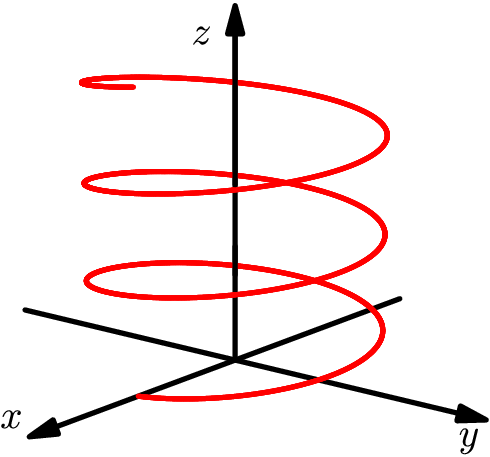
\includegraphics[scale=0.33]{Images/vectorValuedFunctions/Helix}
\end{figure}

\noindent
Since VVFs are essentially multiple single-input single-output functions packaged together, the domain of a VVF is the domain on which all components are defined.\\

\noindent
For example, if $\vec{r}(t)=\langle \tan{t},6t,\ln{\left(16-\right)} \rangle$,
\begin{itemize}
	\item $\tan{t}$ is defined for all real numbers equivalent to $\pm\pi/2$ radians.
	\item $6t$ is defined for all real numbers.
	\item $\ln{\left(16-t^2\right)}$ is defined for $t\in\left(-4,4\right)$.
\end{itemize}
The intersection of these domains is $\left(-4,-\pi/2\right)\cup\left(-\pi/2,\pi/2\right)\cup\left(\pi/2,4\right)$, which is the domain of $\vec{r}(t)$.